\documentclass[12pt, a4paper]{book}
\usepackage[ascii]{inputenc}
\usepackage[left=2cm,right=2cm,top=2cm,bottom=4cm]{geometry}
\usepackage[protrusion=true,expansion=true]{microtype}

\usepackage{amsmath}
\usepackage{amsfonts}
\usepackage{amssymb}
\usepackage{tikz, pgfplots}
\usetikzlibrary{intersections}
\usetikzlibrary{decorations.pathmorphing}
\usepackage{kpfonts}
\usepackage{dsfont}
\pgfplotsset{compat=1.13}
\usepackage{emptypage}

\DeclareMathOperator{\N}{\mathbb{N}}
\DeclareMathOperator{\Q}{\mathbb{Q}}
\DeclareMathOperator{\Z}{\mathbb{Z}}
\DeclareMathOperator{\R}{\mathbb{R}}
\DeclareMathOperator{\C}{\mathbb{C}}
\DeclareMathOperator{\F}{\mathbb{F}}

\usepackage{graphicx}
\usepackage{enumitem}
\setenumerate{}

%
% Some tikz macros useful for graph theory
\tikzset{% 
    vtx/.style={inner sep=2pt,circle,fill=black}
}

%-----------------------------------------------------------------------------------------------------------------
% Some fancy macros // May eventually move these into separate files or something and merge when building template
\renewcommand{\d}[1]{\ensuremath{\operatorname{d}\!{#1}}} % dx macro for integrals
\newcommand{\hess}[1]{\ensuremath{\operatorname{H}\!{#1}}} % Hessian
\newcommand{\diff}[1]{\ensuremath{\operatorname{D}\!{#1}}} % Jacobian
\newcommand{\inner}[2]{\left\langle #1, #2 \right\rangle} % inner product
\newcommand{\norm}[1]{\left\lVert#1\right\rVert} % norm
\newcommand{\cpl}[1]{\overline{#1}} % complement
\renewcommand{\v}[1]{\mathbf{#1}} % vector
\newenvironment{amatrix}[1]{% augumented matrix - make sure to have # columns less than required amount
  \left(\begin{array}{@{}*{#1}{c}|c@{}}
}{%
  \end{array}\right)
}
%-----------------------------------------------------------------------------------------------------------------
% Define theorem environments, along with a custom proof environment
\usepackage[thref, thmmarks,amsmath]{ntheorem}
\newcommand{\itref}[1]{\textit{\thref{#1}}}

\newtheorem{theorem}{Thm.}[section]
\newtheorem{lemma}[theorem]{Lemma}
\newtheorem{definition}[theorem]{Def'n.}
\newtheorem{corollary}[theorem]{Cor.}
\newtheorem{proposition}[theorem]{Prop.}

\theorembodyfont{\upshape}
\newtheorem{remark}[theorem]{Rmk.}
\newtheorem{exercise}[theorem]{Exc.}
\newtheorem{example}[theorem]{Ex.}
\theoremseparator{}
\theoremindent0.0cm
\theoremstyle{nonumberplain}
\theoremheaderfont{\scshape}
\theoremsymbol{$\square$}
\newtheorem{proof}{Proof}

%-----------------------------------------------------------------------------------------------------------------
% Define Document Variables
\newcommand{\assignmentname}{Course Notes}
\newcommand{\classname}{Graph Theory}
\newcommand{\semester}{BSM Fall 2018}

% Define a title page for the document
%----------------------------------------------------------------------------------------------------------------------
% Define headings for each page
\usepackage{fancyheadings}
\pagestyle{fancy}
\lhead{Alex Rutar\\arutar@uwaterloo.ca}
\rhead{\classname: \assignmentname\\\semester}
\cfoot{\thepage}
\setlength{\headheight}{50pt}
%----------------------------------------------------------------------------------------------------------------------
\begin{document}
\pagenumbering{roman}
\begin{titlepage}
    \centering
    \vspace{5cm}
    {\huge\textbf{\assignmentname}\par} % Assignment Name
    \vspace{2cm}
    {\Large\textbf{\classname}\par} % Class
    \vspace{3cm}
    {\Large\textit{Alex Rutar}\par}

    \vfill

% Bottom of the page
    {\large \semester \par} % Due Date
\end{titlepage}
%----------------------------------------------------------------------------------------------------------------------
% \newpage\null\thispagestyle{empty}\textit{This page is left intentionally blank.}\newpage
\pagenumbering{roman}
\tableofcontents
\pagenumbering{arabic}
\chapter{Basic Structure of Graphs}
\section{A Brief Introduction}
\subsection{Basic Definitions}
\begin{definition}
    A \textbf{graph} $G=(V,E)$ consists of a vertex set $V$ and edge set $E$ where $E\subseteq\binom{V}{2}$.
\end{definition}
Note that we write $\binom{V}{2}$ instead of $V\times V$ to make it clear that we cannot have loops and multiple edges.
\begin{definition}
    Two graphs $F$ and $G$ are \textbf{isomorphic} if there exists a bijective mapping $f:V(F)\to V(G)$ such that for every $a,b\in V(F)$: $\{a,b\}\in E(F)\Leftrightarrow \{F(a),f(b)\}\in E(G)$.
\end{definition}
\begin{definition}
    The \textbf{degree} of a vertex $v\in V(G)$ is the number of edges having $v$ as an endpoint.
\end{definition}
\begin{definition}
    The \textbf{neighbourhood} of a graph $U$ is denoted by $N(U):=\{v\in V(G):\exists u\in U\text{ s.t. }\{v,u\}\in E(G)\}$.
\end{definition}
\begin{definition}
    A \textbf{path} is asequence $v_1e_1v_2e_2\ldots v_ie_iv_{i+1}\ldots e_jv_{j+1}$ where each $v_i\in V(G)$ and $e_i=\{v_i,v_{i+1}\}\in E(G)$ where all $v_i$'s are different.
    A \textbf{cycle} is a path in which $v_1=v_{j+1}$.
\end{definition}
\begin{definition}
    The \textbf{complementary graph} of $G=(V,E)$ is $\overline{G}=\left(V,\binom{V}{2}\setminus E\right)$.
\end{definition}
\begin{definition}
    A graph $G$ is called \textbf{connected} if for every $u,v\in V(G)$ there exists a path between $u$ and $v$.
\end{definition}
\begin{definition}
    A connected graph that becomes disconnected with the removal of any edge is called a \textbf{tree}.
    Equivalently, a \textbf{tree} is a graph which is connected and contains no cycle.
\end{definition}
\begin{proposition}
    Any tree on at least two vertices contains at least two vertices of degree 1 (``leaves'').
\end{proposition}
\begin{proof}
    Consider a path of maximal length.
    We claim that both endpoints of $P$ have degree one.
    Suppose for contradiction that an endpoint has greater than one.
    Then the endpoint has another neighbour on the path (in which case we have a cycle), or a unique neighbour (in which case the path is not maximal), a contradiction in either case.
\end{proof}
\begin{proposition}
    A tree on $n$ vertices always has $n-1$ edges.
\end{proposition}
\begin{proof}
    Delete the edges one by one.
    Each time, the number of connected components increases by one.
    After deleting all edges, we have $n$ components, at the beginning, we have one, so we deleted $n-1$ edges.
\end{proof}
We now have an interesting question: how many different trees can be given on $n$ labelled vertices?
To investigate this, we consider the Pr{\"u}fer code. Delete the smallest labelled degree one vertex and write up its unique neighbour's label.
Continue doing this until only one point remains.
The obtained sequences of labels is the Pr\"ufer code.

Properties:
\begin{itemize}[nolistsep]
    \item The length is $n-1$
    \item The last digit must be $n$
\end{itemize}
\begin{theorem}[Cayley]
    The number of different trees on $n$ labelled vertices is $n^{n-2}$.
\end{theorem}
\begin{proof}
    We will show that sequences $x\in\{1,2,\ldots,n\}^{n-1}$ with $x_{n-1}=n$ are in bijective correspondence with the trees on $n$ labelled vertices.
    First, given $a_1a_2\ldots a_{n-2}a_{n-1}$ with $a_{n-1}=n$ we want to decode it.
    Let $b_1,b_2,\ldots,b_{n-1}$ be the sequence of labels of vertices deleted in the order of the indices.
    If we ``decode'' $b_1b_2\ldots b_{n-1}$, we know the tree, since we have the $n-1$ edges $\{a_i,b_i\}$.
    \begin{enumerate}
        \item $b_1:=\min\{k\in\{1,2,\ldots,n\}:k\notin \{a_1,\ldots,a_{n-1}\}\}$
        \item $b_2:=\min\{k\in\{1,2,\ldots,n\}:k\notin \{b_1,a_2,\ldots,a_{n-1}\}\}$
        \item[$(*)$] \fbox{$b_i:=\min\{k\in\{1,2,\ldots,n\}:k\notin \{b_1,\ldots,b_{i-1},a_i,\ldots,a_{n-1}\}\}$}
    \end{enumerate}
    We show that taking any sequence $a_1a_2\ldots a_{n-1}$ with $a_{n-1}=n$ and applying $(*)$ to obtain $b_1,\ldots,b_{n-1}$, the graph we obtain on vertices $1,\ldots,n$ with the $n-1$ edges $\{a_i,b_i\}$ (1) is a tree, and (2) has Pr\"ufer code is just $a_1a_2\ldots a_{n-1}$.

    Note that $(*)$ implies that $\{b_1,b_2,\ldots,b_{n-1},a_{n-1}\}=\{1,2,\ldots,n\}$.
    Define graphs $T_i$ for $i=n-1,n-2,\ldots,2,1$ on the graph spanned by the edges $\{a_{n-1},b_{n-1}\},\{a_{n-2},b_{n-2}\},\ldots,\{a_i,b_i\}$.
    It suffices to prove that $T_i$ is a tree for every $i$ and $b_i$ is its smallest labelled degree 1 vertex.

    We do this by induction.
    Clearly, it is true for $i=n-1$.
    Once it is true for $i=n-1,\ldots,j+1$, we prove this for $i=j$.
    We know that $T_{j+1}$ is a tree, and we wish to add the edge $\{b_j,a_j\}$.
    Thus $b_j\notin V(T_{j+1})=\{b_{j+1},b_{j+2},\ldots,b_{n-1},a_{n-1}\}$ so $b_j$ is indeed degree one; $a_j\in V(T_{j+1})$ and $T_j$ is a tree.
    If $b_j$ was not the smallest degree 1 vertex, then there exists some $k>j$ such that $b_k<b_j$ and $b_k$ has degree one in $T_j$.
    But then $b_k\notin\{b_1,\ldots,b_{j-1},a_j,\ldots,a_{n-1}\}$ so $(*)$ would have chosen it in place of $b_j$, a contradiction.
\end{proof}

\section{Paths, Circuits, and Cycles}
\subsection{Eulerian Circuits}
K\"onigsberg (modern Kaliningrad)
\begin{definition}
    An \textbf{Eulerian circuit} is a closed walk in a graph that contains every edge exactly once.
    An \textbf{Eulerian path} is a walk containing every edge exactly once and not (necessarily) ending at the same vertex.
\end{definition}
Note that we do allow multiple edges between vertices (graph is necessary simple).
We also assume that our graph is connected.
\begin{theorem}[Euler]
    A graph contains an Eulerian circuit if and only if every vertex has even degree.
\end{theorem}
\begin{corollary}
    A graph contains an Eulerian path if and only if all but two vertices have even degree.
\end{corollary}
In both cases, necessity is obvious: every time a path arrives at a vertex, it adds two to the degree since there is a unique edge in and out from the vertex.
Thus for the corollary the only odd vertices can be the endpoints, and for the theorem, there are no endpoints in the path.
\begin{proof}[cor.]
    To see the corollary, first add an edge connecting the two odd degree vertices.
    Then by the theorem, we have an Eulerian circit walk through it so that the added edge is the last one traversed.
    Delete it, and the remaining part of the walk gives our Eulerian path
\end{proof}
\begin{proof}[thm.]
    We can now prove the theorem.
    Consider a maximal walk $P$ on $G$ that does not repeat edges.
    Because of the evenness of all degrees, it must be closed.
    If every edge is contained, it is an Eulerian circuit and we are done.
    If there exists some $e\in E(G)$ that is not in the walk, then by connectedness, there must be a path from a vertex in the walk to an endpoint of $e$.
    Considering a shortest such path (perhaps containing 0 edges), all edges on it are unused so far.
    Now take the starting point of this path on our walk, go through the closed path on our walk, go through the closed walk we have starting here and thus contine on the said path and include $e$, a contradiction.
\end{proof}
\subsection{Hamiltonian Cycles}
\begin{definition}
    A \textbf{Hamiltonian cycle} in a graph is a cycle containing every vertex exactly once.
    A \textbf{Hamiltonian path} is a path that contains every vertex exactly once.
\end{definition}
\subsection{Necessary Conditions}
\begin{proposition}
    If $G$ contains a Hamiltonian cycle, then after deleting any $k$ of its vertices, the remaining graph cannot have more than $k$ components.
    Similarly, if $G$ contains a Hamiltonian path, then deleting any $k$ of it vertices yields a graph with at most $k+1$ components.
\end{proposition}
\begin{proof}
    This can be easily proven by induction.
\end{proof}
Here is a graph for which this condition holds, but does not have a Hamiltonian cycle.
\begin{center}
    \begin{tikzpicture}[
        vtx/.style={circle,radius=0.5pt,fill=black,inner sep=2pt},
        edge/.style={thick}
        ]
        \node[vtx, fill=red] (1a) at (18:2cm){};
        \node[vtx, fill=red] (2a) at (90:2cm){};
        \node[vtx] (3a) at (162:2cm){};
        \node[vtx] (4a) at (234:2cm){};
        \node[vtx] (5a) at (306:2cm){};

        \node[vtx] (1b) at (18:4cm){};
        \node[vtx] (2b) at (90:4cm){};
        \node[vtx] (3b) at (162:4cm){};
        \node[vtx] (4b) at (234:4cm){};
        \node[vtx] (5b) at (306:4cm){};

        \draw[edge] (1b) -- (2b) -- (3b) -- (4b) -- (5b) -- (1b);
        \draw[edge] (1a) -- (1b);
        \draw[edge] (2a) -- (2b);
        \draw[edge] (3a) -- (3b);
        \draw[edge] (4a) -- (4b);
        \draw[edge] (5a) -- (5b);
        \draw[edge] (1a) -- (3a) -- (5a) -- (2a) -- (4a) -- (1a);
    \end{tikzpicture}
\end{center}
The condition holds: delete $k=l_1+l_2$ vertices, where $l_1$ is in the ``outer cycle'' and $l_2$ is in the ``inner cycle''.
(Above, $l_2=2$ and $l_1=0$.)
Then the outer cycle may not fall apart into more than $l_1$ components, the inner cycle may not fall apart into more than $l_2$ component, so if $l_1,l_2>0$.
If $l_1$ or $l_2$ is $0$, then the graph remains connected.

Furthermore, there does not exist a Hamiltonian cycle.
Suppose such a cycle exists, then it is a cycle containing 10 edges.
Colour the alternating edges red and blue.
Thus every vertex is adjacent to a red edge and a blue edge.
Colour the remaining 5 edges white, so every vertex will be the end vertex of exactly 1 white edge.
However, such an edge-coloring is impossible.

Up to isomorphism, the outer edges must be coloured with two of colour 1, two of colour 2, and one of colour 3.
We then fill in the interior edges as required, until the inner cycle, in which we are forced to draw the following edges, yielding our contradiction.
\begin{center}
    \begin{tikzpicture}[
        scale=0.5,
        vtx/.style={circle,radius=0.5pt,fill=black,inner sep=2pt},
        edge/.style={thick}
        ]
        \node[vtx] (1a) at (18:2cm){};
        \node[vtx] (2a) at (90:2cm){};
        \node[vtx] (3a) at (162:2cm){};
        \node[vtx] (4a) at (234:2cm){};
        \node[vtx] (5a) at (306:2cm){};

        \node[vtx] (1b) at (18:4cm){};
        \node[vtx] (2b) at (90:4cm){};
        \node[vtx] (3b) at (162:4cm){};
        \node[vtx] (4b) at (234:4cm){};
        \node[vtx] (5b) at (306:4cm){};

        \draw[edge,draw=blue] (1b) -- (2b);
        \draw[edge,draw=red] (2b) -- (3b);
        \draw[edge,draw=blue] (3b) -- (4b);
        \draw[edge,draw=red] (4b) -- (5b);
        \draw[edge,draw=green] (5b) -- (1b);

        \draw[edge,draw=red] (1a) -- (1b);
        \draw[edge,draw=green] (2a) -- (2b);
        \draw[edge,draw=green] (3a) -- (3b);
        \draw[edge,draw=green] (4a) -- (4b);
        \draw[edge,draw=blue] (5a) -- (5b);

        \draw[edge] (1a) -- (3a);
        \draw[edge] (3a) -- (5a);
        \draw[edge] (5a) -- (2a);
        \draw[edge] (2a) -- (4a);
        \draw[edge] (4a) -- (1a);
    \end{tikzpicture}
    \qquad
    \begin{tikzpicture}[
        scale=0.5,
        vtx/.style={circle,radius=0.5pt,fill=black,inner sep=2pt},
        edge/.style={thick}
        ]
        \node[vtx] (1a) at (18:2cm){};
        \node[vtx] (2a) at (90:2cm){};
        \node[vtx] (3a) at (162:2cm){};
        \node[vtx] (4a) at (234:2cm){};
        \node[vtx] (5a) at (306:2cm){};

        \node[vtx] (1b) at (18:4cm){};
        \node[vtx] (2b) at (90:4cm){};
        \node[vtx] (3b) at (162:4cm){};
        \node[vtx] (4b) at (234:4cm){};
        \node[vtx] (5b) at (306:4cm){};

        \draw[edge,draw=blue] (1b) -- (2b);
        \draw[edge,draw=red] (2b) -- (3b);
        \draw[edge,draw=blue] (3b) -- (4b);
        \draw[edge,draw=red] (4b) -- (5b);
        \draw[edge,draw=green] (5b) -- (1b);

        \draw[edge,draw=red] (1a) -- (1b);
        \draw[edge,draw=green] (2a) -- (2b);
        \draw[edge,draw=green] (3a) -- (3b);
        \draw[edge,draw=green] (4a) -- (4b);
        \draw[edge,draw=blue] (5a) -- (5b);

        \draw[edge,draw=blue] (1a) -- (3a);
        \draw[edge,draw=red] (3a) -- (5a);
        \draw[edge,draw=red] (5a) -- (2a);
        \draw[edge] (2a) -- (4a);
        \draw[edge,draw=blue] (4a) -- (1a);
    \end{tikzpicture}
\end{center}
\subsection{Sufficient Conditions}
\begin{theorem}[Dirac, 1952]
    If $G$ is a graph on $n$ vertices, with every degree being at least $\frac{n}{2}$, then $G$ contains a Hamiltonian cycle.
\end{theorem}
As a fun fact, this is not Paul Dirac, but rather Gabriel Andrew Dirac (Paul Dirac's stepson).
Note that we must have $f(n)\geq n/2$.
If not, then the graph composed of two disconnected components $K_{n/2}$ has degree $n/2-1$ everywhere but does not have a hamiltonian cycle.
We also have the following stronger theorem:
\begin{theorem}[Ore, 1960]
    If $G$ is a graph on $n$ vertices such that for every nonadjacent pair of vertices $u,v\in V(G)$, $d(u)+d(v)\geq n$ is satisfied, then $H$ contains a Hamiltonian cycle.
\end{theorem}
\begin{proof}
    Assume for contradiction we have $G_0$ satisfying the condition but does not have a Hamiltonian cycle.
    Saturate $G_0$ go obtain $G$: if two vertices are non-adjacent and connecting them still creates a Hamiltonian cycle, then connect them.
    Observe that the new graph is still a counterexample since the condition will obviously remain true.
    Do this maximally, so that the addition of any edge would create a Hamiltonian cycle.

    Now, if $a,b\in V(G)$ are non-adjacent in $G$, then there exists a Hamiltonian path starting at $a$ and ending at $b$.
    Consider such a Hamiltonian path $(x_1,x_2,\ldots,x_n)$.
    \begin{center}
        \begin{tikzpicture}
            \node[circle,inner sep=2pt,fill=black,label=below:{$a=x_1$}] (x1) at (0,0){};
            \node[circle,inner sep=2pt,fill=black,label=above:{$x_2$}] (x2) at (1,0){};
            \node[circle,inner sep=2pt,fill=black,label=above:{$x_3$}] (x3) at (2,0){};
            \node[circle,inner sep=2pt,fill=black,label=above:{$x_{i-1}$}] (xim1) at (5,0){};
            \node[circle,inner sep=2pt,fill=black,label=above:{$x_i$}] (xi) at (6,0){};
            \node[circle,inner sep=2pt,fill=black,label=above:{$x_{i+1}$}] (xip1) at (7,0){};
            \node[circle,inner sep=2pt,fill=black,label=above:{$x_{n-1}$}] (xnm1) at (10,0){};
            \node[circle,inner sep=2pt,fill=black,label=above:{$x_{n}=b$}] (xn) at (11,0){};

            \node[inner sep=0pt] (a) at (3,0){};
            \node[inner sep=0pt] (b) at (4,0){};
            \node[inner sep=0pt] (c) at (8,0){};
            \node[inner sep=0pt] (d) at (9,0){};

            \draw (x1) -- (x2) -- (x3) -- (a);
            \draw[dotted] (a) -- (b);
            \draw (b) -- (xim1) -- (xi) -- (xip1) -- (c);
            \draw[dotted] (c) -- (d);
            \draw (d) -- (xnm1) -- (xn);

            \draw plot [smooth, tension=1.4] coordinates { (x1) (3,1) (xi)};
            \draw [dashed] plot [smooth, tension=1.4] coordinates { (xim1) (8,-1) (xn)};
            \node (X) at (8,-1){\large $\times$};
        \end{tikzpicture}
    \end{center}
    Observe that if $\{a,x_i\}\in E(G)$, then $\{a,x_{i-1}\}\notin E(G)$ or we would have a Hamiltonian cycle given by $(a,x_i,x_{i+1},\ldots,b,x_{i-1},x_{i-2},\ldots,a)$.
    This implies that $d(b)\leq n-1-d(a)$: for each neighbour of $a$, there is a distinct non-neighbour of $b$.
    But this is a contradiction since $d(a)+d(b)\leq n-1$ while $\{a,b\}\notin E(G)$ and $G$ does not satisfy the condition.
\end{proof}
\begin{theorem}[P\'osa, 1962]
    Let $G$ be a graph on $n$ vertiecs with degrees $d_1\leq d_2\leq\cdots\leq d_n$.
    Then for every $k<n/2$, we have $d_k\geq k+1$, then $G$ contains a Hamiltonian cycle.
\end{theorem}
\begin{theorem}[Chv\'atal, 1972]
    \hfill
    \begin{enumerate}[nolistsep, label=(\roman*)]
        \item Let $G$ be a graph on $n$ vertices with degrees $d_1\leq d_2\leq\cdots\leq d_n$.
            Assume that whenever for some $k<n/2$, if we have $d_k\leq k$, $d_{n-k}\geq n-k$.
            Then $G$ contains a Hamiltonian cycle.
        \item Assume that the number $d_1'\leq d_2'\leq\cdots d_n'$ do not satisfy the implication.
            Then there exists a graph $G$ with degrees $d_1\leq d_2\leq\cdots\leq d_n$ such that $d_i\geq d_i'$ and $G$ has no Hamiltonian cycle.
    \end{enumerate}
\end{theorem}
\begin{proof}
    \begin{enumerate}[label=(\roman*)]
        \item Assume that the statement is false, consider a counterexample $G_0$, and saturate it to obtain $G$.
            This works: if an edge can be added without creating a Hamiltonian cycle; then after adding we will still have a counterexample, the validity of the condition cannot be destroyed by adding an edge.
            From Ore's proof, we know that for every $a,b\in V(G)$ that are non-adjacent, there exists a Hamiltonian path from $a$ to $b$ and $d(a)+d(b)\leq n-1$.
            Consider an $a,b\in V(G)$, $\{a,b\}\notin E(G)$ pair for which $d(a)+d(b)$ is maximal
            \begin{center}
                \begin{tikzpicture}
                    \node[circle,inner sep=2pt,fill=black,label=below:{$a=x_1$}] (x1) at (0,0){};
                    \node[circle,inner sep=2pt,fill=black,label=above:{$x_2$}] (x2) at (1,0){};
                    \node[circle,inner sep=2pt,fill=black,label=above:{$x_3$}] (x3) at (2,0){};
                    \node[circle,inner sep=2pt,fill=black,label=above:{$x_{i-1}$}] (xim1) at (5,0){};
                    \node[circle,inner sep=2pt,fill=black,label=above:{$x_i$}] (xi) at (6,0){};
                    \node[circle,inner sep=2pt,fill=black,label=above:{$x_{i+1}$}] (xip1) at (7,0){};
                    \node[circle,inner sep=2pt,fill=black,label=above:{$x_{n-1}$}] (xnm1) at (10,0){};
                    \node[circle,inner sep=2pt,fill=black,label=above:{$x_{n}=b$}] (xn) at (11,0){};

                    \node[inner sep=0pt] (a) at (3,0){};
                    \node[inner sep=0pt] (b) at (4,0){};
                    \node[inner sep=0pt] (c) at (8,0){};
                    \node[inner sep=0pt] (d) at (9,0){};

                    \draw (x1) -- (x2) -- (x3) -- (a);
                    \draw[dotted] (a) -- (b);
                    \draw (b) -- (xim1) -- (xi) -- (xip1) -- (c);
                    \draw[dotted] (c) -- (d);
                    \draw (d) -- (xnm1) -- (xn);

                    \draw plot [smooth, tension=1.4] coordinates { (x1) (3,1) (xi)};
                    \draw [dashed] plot [smooth, tension=1.4] coordinates { (xim1) (8,-1) (xn)};
                    \node (X) at (8,-1){\large $\times$};
                \end{tikzpicture}
            \end{center}
            We may assume $d(a)\leq d(b)$.
            Then we have $d(a)\leq\frac{n-1}{2}<\frac{n}{2}$.
            For notation, $h=d(a)$.
            We claim that $d_h\leq h<\frac{n}{2}$.
            We show $d_h\leq h$.
            
            From the Ore proof argument, we know that $b$ has at least as many non-neighbours as many neighbours $a$ has, i.e. $h$.
            Each of these non-neighbours $x$ of $b$ could have been chosen for $a$ (as a non-adjacent pair for $b$), but it was not, do $d(x)\leq d(a)=h$.
            Thus there exists an index greater than or equal to $h$ with degree less than or equal to $h$.
            This exactly means $d_h\leq h$, and we have our claim.

            Thus by our condition, $d_{n-h}\geq n-h$, so there exist $h+1$ degrees $\geq n-h$.
            Then by the Pidgeonhole Principle, there exists at least one non-neighbour of $a$, call it $y$, that has degree $\geq n-h$.
            But then $a,y$ is a non-adjacent pair with $d(a)+d(y)\geq h+n-h=n>d(a)+d(b)$, a contradiction to the choice of $a,b$.
        \item Assume $d_1'\leq\cdots\leq d_n'$ violates our condition.
            Then we have $k$ so that $d'_k\leq k<n/2$ and $d'_{n-k}\leq n-k-1$.
            Fix such a $k$, then
            \[d_1'\leq d_2'\leq\cdots\leq d_k'\leq k\]
            \[d_{k+1}'\leq d_{k+2}'\leq\cdots\leq d_n'\leq n-k-1\]
            and clearly, $d_{n-k+1}'\leq\cdots\leq d_n'\leq n-1$.
            Set $d_1=d_2=\cdots=d_k:= k$, $d_{k+1},d_{k+2}=\cdots=d_{n-k}:=n-k-1$ and $d_{n-k+1}=\cdots=d_n:=n-1$.
            Thus it is enough to show a graph with these degrees and no Hamiltonian cycle.
            Here is such a graph:
            \begin{center}
                \begin{tikzpicture}
                    \draw (0,0) ellipse (1cm and 2cm) node{$k$};
                    \draw (3,0) ellipse (1cm and 2cm) node{$k$};
                    \draw (6,0) ellipse (1cm and 2cm) node{$n-2k$};
                    \draw[dashed] (4.5,0) ellipse (3cm and 3cm);
                    \draw[dashed] (1.5,0) ellipse (3cm and 3cm);
                    \node[below] (a) at (1.5,-3){$K_{k,k}$};
                    \node[below] (b) at (4.5,-3){$K_{n-k}$};
                \end{tikzpicture}
            \end{center}
            It can be verified that the degrees in the first compoent are $k$, second are $n-1$ and third are $n-k-1$.
            Furthermore, the graph has no Hamiltonian cycle.
            Remove the $k$ vertices of degree $N-1$, and we are left with $k+1$ components, so the necessary condiion for Hamiltonicity we had is violated.
    \end{enumerate}
\end{proof}
\section{Matchings}
\begin{definition}
    A \textbf{matching} in a graph is a subset $M\leq E(G)$ such that all edges in $E(G)$ are independent, meaning that if $e,f\in M$, then $e\cap f=\emptyset$.
\end{definition}
\begin{definition}
    A matching is \textbf{maximal} if no edges can be added to it, \textbf{maximum} if there is no larger matching, and \textbf{perfect} if it covers all the vertices.
\end{definition}
All perfect matchings are maximum, and all maximum matchings are maximal.
Below we have two matchings: a maximal matching in red, and a perfect and maximum matching in blue.
\begin{center}
    \begin{tikzpicture}[scale=2]
        \node[vtx] (a) at (0,0){};
        \node[vtx] (b) at (1,0){};
        \node[vtx] (c) at (0.5,0.5){};
        \node[vtx] (d) at (1.2,-0.4){};
        \node[vtx] (e) at (2,0){};
        \node[vtx] (f) at (2,0.5){};

        \draw[red,thick,dashed] (a) -- (b);
        \draw[red,thick,dashed] (c) -- (e);

        \draw[blue,thick,dashed] (a) -- (c);
        \draw[blue,thick,dashed] (e) -- (f);
        \draw[blue,thick,dashed] (b) -- (d);

        \draw[thick] (b) -- (c);
        \draw[thick] (b) -- (f);
    \end{tikzpicture}
\end{center}
\subsection{Bipartite Matchings}
\begin{definition}
    A graph $G=(V,E)$ is \textbf{bipartite} if $V=A\cup B$ with $A\cap B=\emptyset$, and for all $e\in E(G)$, $|e\cap A|=|e\cap B|=1$ (every edge has an endpoint in $A$ and an endpoint in $B$).
\end{definition}
\begin{theorem}
    A graph is bipartite if and only if it contains no odd cycles.
\end{theorem}
\begin{proof}
    The forwards direction is easy.
    Thus suppose $G$ contains no odd cycle.
    Observe that we can argue separately for each component, so we can assume $G$ is connected.
    Thus $G$ has a spanning tree $T\subseteq G$ such that $V(T)=V(G)$.

    Note that $T$ is bipartite: choose a starting node to belong to $A$, then there is a unique way to partition the vertices into $A$ and $B$.
    Now put back the edges.
    If there is an edge between two vertices of the same class, then the endpoints have even distance from each other, so that when adding the edge we have an odd cycle.

    See the diagram below for an illustration of this idea (the path is dotted, the added edge is blue and dashed).
\end{proof}
\begin{center}
    \begin{tikzpicture}[scale=2]
        \node[vtx,fill=blue] (1a) at (0,3){};

        \node[vtx,fill=red] (2a) at (-0.5,2.5){};
        \node[vtx,fill=red] (2b) at (0.5,2.5){};

        \node[vtx,fill=blue] (3a) at (0,2){};
        \node[vtx,fill=blue] (3b) at (1,2){};

        \node[vtx,fill=red] (4a) at (0.5,1.5){};
        \node[vtx,fill=red] (4b) at (1.5,1.5){};

        \node[vtx,fill=blue] (5a) at (0,1){};
        \node[vtx,fill=blue] (5b) at (0.5,1){};
        \node[vtx,fill=blue] (5c) at (1,1){};

        \draw (1a) -- (2a);
        \draw (1a) -- (2b);

        % \draw (2b) -- (3a);
        % \draw (2b) -- (3b);

        % \draw (3b) -- (4a);
        \draw (3b) -- (4b);

        % \draw (4a) -- (5a);
        \draw (4a) -- (5b);
        \draw (4a) -- (5c);

        \draw[dashed, blue] (3a) -- (5a);
        \draw[thick, dotted, black] (3a) -- (2b) -- (3b) -- (4a) -- (5a);
    \end{tikzpicture}
\end{center}
\begin{theorem}[Hall]
    A bipartite graph $G=(A,B;E)$ admits a matching covering $A$ if and only if for every $U\subseteq A$, $V\subseteq B$, $|N(U)|\geq |U|$.
\end{theorem}
\begin{corollary}[Frobenius]
    A bipartite graph $G=(A,B;E)$ contains a perfect matching if and ony if Hall's condition holds and $|A|=|B|$.
\end{corollary}
We need a few definitions to prove these theorems.
\begin{definition}
    Given a matching $M\subseteq E(G)$, an \textbf{alternating path} (with respect to $M$) is a path such that every second edge belongs to $M$.
\end{definition}
\begin{definition}
    An alternating path beginning and ending at vertices not covered by any matching edge (from $M$) is called an \textbf{augumenting path}.
\end{definition}
\begin{proof}[Hall]
    Let $M\subseteq E(G)$ be a matching in a bipartite graph $G=(A,B;E)$ for which there exists no augumenting path.
    Assume $M$ does not cover $A$, let the set of vertices in $A$ not covered by $M$ be called $W$, so $W\neq\emptyset$.
    Let $T\subseteq B$ be the set of vertices one can go to from $W$ via an alternating path (w.r.t. $M$).
    \begin{center}
        \begin{tikzpicture}
            % draw main ellipses, labels
            \draw[thick] (0.5,3) ellipse (5.5cm and 1cm);
            \draw[thick] (0.5,-1) ellipse (5.5cm and 1cm);
            \node (A) at (6.5,3){\large$A$};
            \node (B) at (6.5,-1){\large$B$};
            \node (M) at (-4,1){\large$M$};

            % draw ellipse for W
            \draw (3,3) ellipse (1.4cm and 0.5cm);
            \node(W) at (2.5,4.6){\large$W$};
            \draw (W) -- (3,3.6);

            % draw rectangle for T'
            \draw[thick] (-1.4,2.5) rectangle (1.4,3.5);
            \node(Tp) at (-0.5,4.7){\large$T'$};
            \draw (Tp) -- (0,3.6);

            % draw rectangle for T
            \draw[thick] (-1.4,-1.5) rectangle (1.4,-0.5);
            \node(Tp) at (-0.5,-2.7){\large$T$};
            \draw (Tp) -- (0,-1.6);

            % graph vertices
            \node[vtx] (a1) at (-3,3){};
            \node[vtx] (a2) at (-2,3){};
            \node[vtx] (a3) at (-1,3){};
            \node[vtx] (a4) at (0,3){};
            \node[vtx] (a5) at (1,3){};
            \node[vtx, inner sep=1pt] (a6) at (2,3){};
            \node[vtx, inner sep=1pt] (a7) at (3,3){};
            \node[vtx, inner sep=1pt] (a8) at (4,3){};

            \node[vtx] (b1) at (-3,-1){};
            \node[vtx] (b2) at (-2,-1){};
            \node[vtx] (b3) at (-1,-1){};
            \node[vtx] (b4) at (0,-1){};
            \node[vtx] (b5) at (1,-1){};
            \node[vtx, inner sep=1pt] (b6) at (2,-1){};
            \node[vtx, inner sep=1pt] (b7) at (3,-1){};

            % matching
            \draw[thick] (a1) -- (b1);
            \draw[thick] (a2) -- (b2);
            \draw[thick] (a3) -- (b3);
            \draw[thick] (a4) -- (b4);
            \draw[thick] (a5) -- (b5);

            % not in matching
            \draw[thin, dashed] (b3) -- (a4);
            \draw[thin, dashed] (b3) -- (a5);
            \draw[thin, dashed] (b4) -- (a3);
            \draw[thin, dashed] (b4) -- (a8);
            \draw[thin, dashed] (b5) -- (a7);
        \end{tikzpicture}
    \end{center}

    Every $v\in T$ is covered by $M$, otherwise there would exist an augumenting path w.r.t. $M$, but we assumed it does not exist.
    Let $T'$ be the set of vertices in $A$ that are the pairs of the vertices in $T$ according to $M$.
    We have $|T'|=|T|$, and we claim that $U=T'\cup W$ violates the condition.
    In particular, we show that $N(T'\cup W)\subseteq T$.
    Indeed, $N(T'\cup W)=N(T')\cup N(W)$.
    \begin{enumerate}[nolistsep]
        \item $N(W)\subseteq T$ since any single edge starting at some $w\in W$ can ... as an alternating path, so its other end must be in $T$ by definition (of $T$).
        \item $N(T')\subseteq T$.
            Let $v\in T'$; then $v$ has a matched pair $v\in T$ (i.e., $\{v,v'\}\in M$) and since $v\in T$, there exists an alternating path from $W$ to $r$.
            Thus path does not contain the matching edge $\{v,v'\}$, so $P\cup\{v,v'\}$ is still an alternating path and if $z$ is a neighbour of $v'$ not yet in the path, then $P\cup\{v,v'\}\cup \{v',z\}$ is as an alternating path that goes from $W$ to $z$.
            Since $z\in T$ by definition, we have $N(T')\subseteq T$.
    \end{enumerate}
    Thus $N(T'\cup W)\subseteq T$.
    But $|T|=|T'|<|T'|+|W|=|T'\cup W|$, violating Hall's condition.
    Thus if no subset of $A$ violates the condition, then there still exists an augumenting path, so one can increase the size of $M$.
    If we cannot do this anymore, then either the condition is violated, or $W=\emptyset$ and $M$ contains every vertex in $A$.
\end{proof}
\subsection{Minimax: Matchings and Coverings}
\begin{definition}
    The \textbf{matching number} $\nu(G)$ of a graph $G$ is the size of the number of edges in a maximum matching.
\end{definition}
\begin{definition}
    The \textbf{(vertex) covering number} $\tau(G)$ of a graph $G$ is the minimum number of vertices that ``cover'' all edges, i.e. has the property that every edge is represented by at least one of them.
\end{definition}
Note that $\nu(G)\leq\tau(G)$ since every edge in a matching needs a separate point in a vertex covering.
Strict inequality can occur; for example any odd cycle.
This is an example of a ``minimax'' property: if equality holds, then both values must be optimal.
\begin{theorem}[K\"onig]
    If $G$ is bipartite, then $\tau(G)=\nu(G)$.
\end{theorem}
\begin{proof}
    Let $M$ be a maximum matching in a bipartite graph $G$, i.e. $|M|=\nu(G)$.
    Define $W,T,T'$ as in the proof of Hall's Theorem.
    We proved that $N(T'\cup W)=T$.
    This implies that the vertices in $T$ cover all edges with an endpoint in $T'\cup W$.
    Since every edge has an endpoint in $A$, the remaining edges are covered by the vertices in $A\setminus(T'\cup W)$.
    Thus $\tau(G)\leq |T|+|A\setminus(T'\cup W)|=|M|$ and equality holds.
\end{proof}
\subsection{Tutte's Theorem and Applications}
\begin{theorem}[Tutte]
    A graph $G$ contains a perfect matching iff for any $S\subseteq V(G)$, we must have $c_{\text{odd}}(G\setminus S)\leq |S|$.
    $c_{\text{odd}}$ denotes the number of components with odd size.
\end{theorem}
\begin{proof}[Lov\'asz]
    $(\Rightarrow)$ In the odd components, (i.e. components with an odd number of vertices) of $G\setminus S$ at least one vertex must be matched to a vertex in $S$.
    Thus $|S|$ cannot be smaller than the number of such components, which is $c_{\text{odd}}(G\setminus S)$.

    $(\Leftarrow)$ Assume the statement is false and let $G_0$ be a counterexample.
    Saturate $G_0$: add edges until impossible without creating a perfect matching.
    We must show that we cannot increase the number of odd components by adding edges.
    If the edge joins two even components, then we get a new even component; or two odd components, and we have a new even component; or an even and an odd component, and we have a new odd component.
    In any case, the number of odd components stays the same and the graph remains a counterexample.
    Let the saturated graph be denoted by $G$.

    It is sufficient to prove that deleting the points of $G$ that are connected to all other vertex, the remaining graph is the union of vertex disjoint graphs.
    Suppose this is true: then in $G\setminus S$ (where $S:=\{v\in V(G):\{u,v\}\in E(G)\forall u\in V(G),u\neq v\}$), we can create a perfect matching within each even component and every vertex except one in the odd components (since the components are complete).
    We can then pair these components arbitrarily in $S$, since $S$ is connected to everything.
    Then there must be only an even number of vertices in $S$ remaining, or $G$ violates the condition with $S=\emptyset$; and these vertices are mutually connected.

    Thus assume this claim is not true.
    Then there exist vertices $a,b,c\in V(G)$ inducing a path on $3$ vertices.
    Also, $c\notin S$.
    Thus we have some $d\in V(G)$ so that $\{c,d\}\notin E(G)$.
    \begin{center}
        \begin{tikzpicture}[
                scale=3,
                sqg/.style={decorate, decoration={snake, amplitude=1.1}}
            ]
            \node[vtx,label=below:{$a$}] (a) at (0,0){};
            \node[vtx,label=below:{$b$}] (b) at (1,0){};
            \node[vtx,label=above:{$c$}] (c) at (0.5,0.75){};
            \node[vtx,label=above:{$d$}] (d) at (1,0.75){};
            \node[vtx] (e) at (1.5,0){};
            \node[vtx] (f) at (1,-0.75){};
            \node[vtx] (g) at (0.5,-0.75){};
            \node[vtx] (h) at (0,-0.75){};
            \node[vtx] (i) at (-0.5,0){};
            \node[vtx] (j) at (0,0.75){};

            \draw[thick] (a) -- (c) -- (b);
            \draw[thick,dashed] (a) -- (b);
            \draw[thick,dashed] (c) -- (d);
            \draw[thick] (d) -- node[above right]{\small$\in M_1$}(e);
            \draw[thick,sqg] (e) -- node[below right]{\small$\in M_2$}(f);
            \draw[thick] (f) -- node[below]{\small$\in M_1$}(g);
            \draw[thick,sqg] (g) -- node[below]{\small$\in M_2$}(h);
            \draw[thick] (h) -- node[below left]{\small$\in M_1$}(i);
            \draw[thick,sqg] (i) -- node[above left]{\small$\in M_2$}(j);
            \draw[thick] (j) -- node[above]{\small$\in M_1$}(c);
        \end{tikzpicture}
    \end{center}
    Since $G$ is saturated, there exists a perfect matching $M_1$ in $G\cup\{\{a,b\}\}$ and $M_2$ in $G\cup\{\{c,d\}\}$.
    Start a walk from $d$ along alternating edges in $M_1$ and $M_2$.
    Let $P$ be a longest such path.
    Then $P$ can end only in $a$, $b$, or $c$.

    First consider that we end in $c$.
    Then the edge set $M_2\setminus P\cup(M_1\cap P)$ forms a perfect matching.
    If $P$ ends in $a$ or $b$, then without loss of generality we may assume it ends in $a$.
    Now consider the cycle $C=P\cup\{a,c\}\cup\{c,d\}$.
    Then $M_2\setminus C\cup (M_1\cap C)$ is a perfect matching.
    Thus a perfect matching exists in $G$, so the claim is true, so the theorem holds.
\end{proof}

\end{document}
